\chapter{Fonctions - Comparaison et ordres de grandeur.}\label{comp/ord}
\section{Rappels}\label{comp/ord:reminders}
\subsection{Fonctions à variables Réelles}

\section{Comparaison des fonctions}\label{comp/ord:comp}
\subsection{Adhérence}
\begin{definition}
    Adhérence :\\
    Soit \(\mathcal{D}\subset\mathbb{R}\) et \(f:\mathcal{D}\rightarrow\mathbb{R}\)\\
    L'adhérence de \(\mathcal{D}\) note \(\overline{\mathcal{D}}\), est le plus petit (au sens de l'inclusion) fermé qui contient \(\mathcal{D}\).
\end{definition}
\begin{example}
    .\\
    Si \(\mathcal{D} = ]1;2[\) alors \(\overline{\mathcal{D}} = [1;2]\)\\
    Si \(\mathcal{D} = ]-\infty;2[\) alors \(\overline{\mathcal{D}} = ]-\infty;2]\)\\
    Si \(\mathcal{D} = ]1;+\infty[\) alors \(\overline{\mathcal{D}} = [1;+\infty[\)
    \begin{Note}
        Notation :\\
        L'infini est exclu de \(\overline{\mathcal{D}}\) car l'adhérence d'un sous-ensemble de \(\mathbb{R}\) est un sous-ensemble de \(\mathbb{R}\) et donc ne peut contenir l'infini \autocite{TODO}.
    \end{Note}
\end{example}
\begin{Todo}
    Hors programme :\\
    Détailler l'adhérence d'un point de vue topologique, dans la section : \\\textbf{Hors programme \cref{comp/ord:further}}\par
    Voir : \\\url{https://en.wikipedia.org/wiki/Closure_(topology)}
\end{Todo}

\subsection{Limites}
Soit \(f\) définie sur \(\mathcal{D}\) avec :
\begin{flalign}
    a&\in \overline{\mathcal{D}}\\
    \ell&\in\mathcal{D}
\end{flalign}
On dit que \(f\) a pour limite \(\ell\) quand \(x\) tend vers \(a\) si :
\begin{flalign}
&\forall\epsilon>0,\exists\eta>0,\forall x\in\mathcal{D},|x-a|<\eta\Rightarrow|f(a)-\ell|<\epsilon\\
&\text{On note } f(x) \xrightarrow[x\to a]{}\ell
\end{flalign}

\subsection{Fonctions négligeables}
Soient \(f\) et \(g\) deux fonctions définies sur \(\mathcal{D}\) et \(a\in\mathcal{D}\)
\begin{definition}
    négligeable\\
    On dit que \(f\) est négligeable devant \(g\) quand \(x\) tend vers \(a\) ssi :
    \begin{equation}
        \frac{f(x}{g(x)}\xrightarrow[x\to a]{}0
    \end{equation}
    On note alors :
    \begin{equation}
        f(x)=\underset{x\to a}{o}g(x)
    \end{equation}
\end{definition}
\begin{example}
    .\\
    \begin{figure}[H] % Met le graphique dans un environnement figure
        \centering
        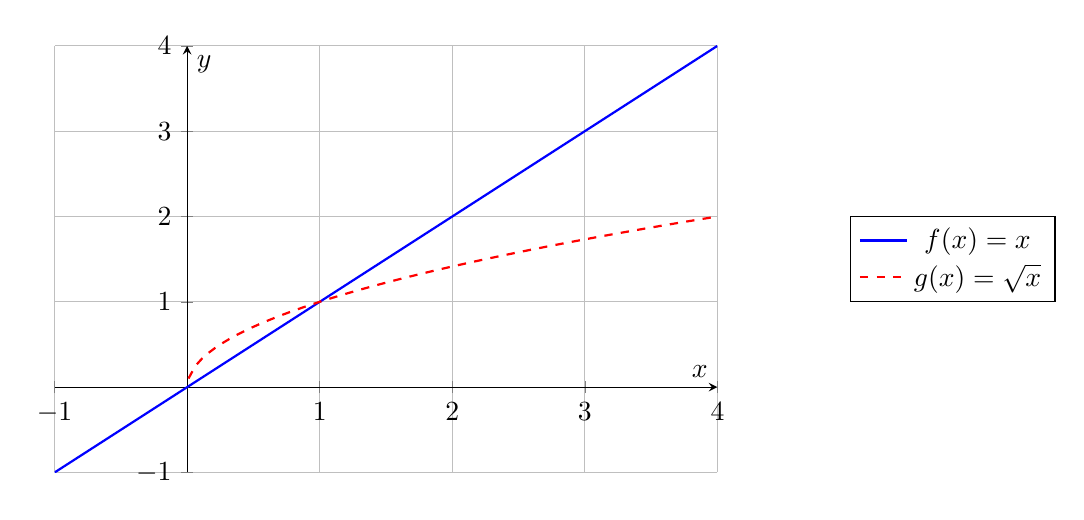
\begin{tikzpicture}
            \begin{axis}[
                axis lines = center,
                xlabel = {$x$},
                ylabel = {$y$},
                legend style={at={(1.2,0.5)}, anchor=west}, % Légende à droite
                domain=-1:4, % Domaine des fonctions
                samples=100, % Plus de points pour des courbes lisses
                grid=both, % Grille sur le graphique
                width=10cm, height=7cm % Taille du graphique
            ]
                % Dessiner f(x) = x
                \addplot[blue, thick] {x};
                \addlegendentry{$f(x) = x$}
                
                % Dessiner g(x) = sqrt(x)
                \addplot[red, thick, dashed] {sqrt(x)};
                \addlegendentry{$g(x) = \sqrt{x}$}
            \end{axis}
        \end{tikzpicture}
        \caption{Graph des fonctions \(f(x)\) et \(g(x)\)}
    \end{figure}
    
    \textbf{En 0 :}
    \begin{equation}
        \frac{f(x)}{g(x)}=\frac{x}{\sqrt{x}}=\sqrt{x}\xrightarrow[x\to0]{}0\text{ donc }f(x)=\underset{x\to 0}{o}g(x)\\
    \end{equation}
    
    \textbf{En \(+\infty\) :}
    \begin{equation}
            \frac{g(x)}{f(x)}=\frac{\sqrt{x}}{x}=\frac{1}{\sqrt{x}}\xrightarrow[x\to+\infty]{}0\text{ donc }g(x)=\underset{x\to+\infty}{o}f(x)
    \end{equation}
\end{example}

\begin{Note}
    Exemples à connaître :\\
    On compare les fonctions :
    \begin{align}
        &x\mapsto\left(\ln x\right)^\alpha &,\alpha>0\\
        &x\mapsto x^\beta&,\beta>0\\
        &x\mapsto\gamma^x=e^{x\ln\gamma}&,\gamma>1
    \end{align}
        \begin{figure}[H]
        \centering
        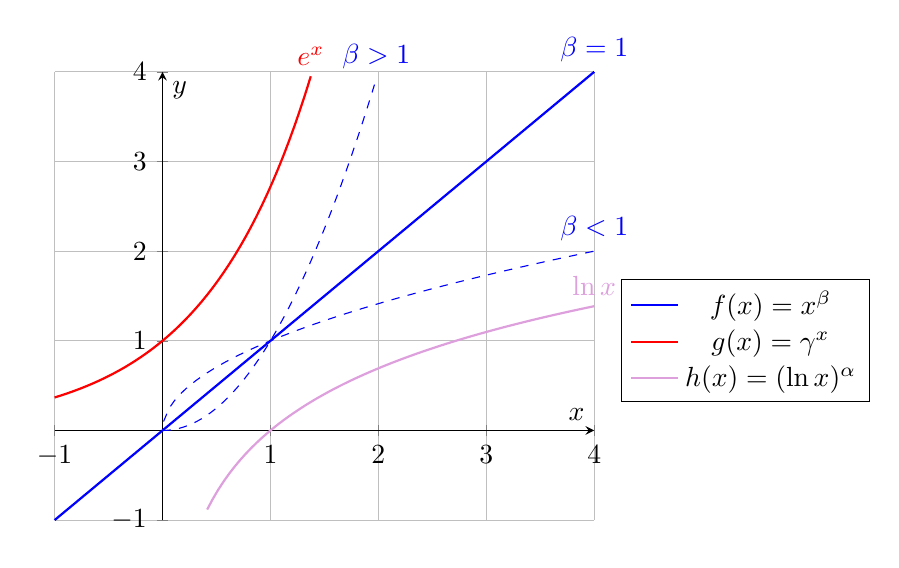
\begin{tikzpicture}
            \begin{axis}[
                axis lines = center,
                xlabel = {$x$},
                ylabel = {$y$},
                legend style={at={(1.05,0.4)}, anchor=west},
                domain=-1:4,
                samples=100,
                grid=both,
                ymin=-1, ymax=4,
                restrict y to domain=-1:4,
                clip=false
            ]
                % x^\beta
                \addplot[blue, thick, line legend] {x} node[above,pos=1] {$\beta=1$}; % label for beta = 1
                \addplot[blue, dashed, domain=0:4, forget plot] {x^2} node[above,pos=1] {$\beta>1$}; % label for beta > 1
                \addplot[blue, dashed, forget plot] {sqrt(x)} node[above,pos=1] {$\beta<1$}; % label for beta < 1
                \addlegendentry{$f(x) = x^\beta$}

                \addplot[red, thick, line legend] {exp(x)} node[above,pos=1] {$e^x$};
                \addlegendentry{$g(x) = \gamma^x$}

                \addplot[Plum, thick, line legend] {ln(x)} node[above,pos=1] {$\ln x$};
                \addlegendentry{$h(x)=(\ln x)^\alpha$}
            \end{axis}
        \end{tikzpicture}
        \caption{Graph de valeurs remarquables\\ des fonctions listées plus haut}
    \end{figure}

    \textbf{En \(+\infty\) :}
    \begin{flalign}
        (\ln x)^\alpha=\underset{x\to+\infty}{o}\left(x^\beta\right)&\text{, \emph{ie.}} \frac{(\ln x)^\alpha}{x^\beta}\xrightarrow[x\to+\infty]{}0\\
        x ^\beta=\underset{x\to+\infty}{o}\left(\gamma^x\right)&\text{, \emph{ie.}} \frac{x^\beta}{\gamma^x}\xrightarrow[x\to+\infty]{}0
    \end{flalign}
\end{Note}

\begin{remark}
    Quelques équivalences :\\
    Un polynôme est équivalent a son monôme de plus haut degré quand \(x\) tend vers \(+\infty\) :
    \begin{flalign}
        P(x)&=2x+7x^2-8x^3\\
        P(x)&\underset{x\to+\infty}{\sim}-8x^3\\
        P(x)&\underset{x\to0}{\sim}2x
    \end{flalign}
    \begin{equation}
        \sin{x}\underset{x\to0}{\sim}x
    \end{equation}
    \begin{equation}
        \ln{1+x}\underset{x\to0}{\sim}x
    \end{equation}
\end{remark}

\subsection{Continuité}
\begin{definition}
    Continuité\\
    \(f\) est continue en \(x\) ssi :
    \begin{equation}
        f(x)\underset{x\to\alpha}{\rightarrow}f(\alpha)
    \end{equation}
     Continuité des fonctions \(f+g, f\circ g, f\cdot g, \frac{f}{g}\) vue en L1.
\end{definition}
\begin{Todo}
    Rappels\\
    Mettre les démonstrations de continuité des fonctions ci-dessus dans la section \Cref{comp/ord:reminders}.
\end{Todo}

\subsection{Dérivabilité}
\begin{definition}
    Dérivabilité\\
    \(f\) est dérivable en \(\alpha\) ssi :
    \begin{equation}
        \frac{f(x)-f(\alpha)}{x-\alpha}\underset{x\to\alpha}{\rightarrow}\ell\in\mathbb{R}
    \end{equation}
    Dérivabilité des fonctions \(f+g, f\circ g, f\cdot g, \frac{f}{g}\), dérivées successives vue en L1.
\end{definition}
\begin{Todo}
    Rappels\\
    Mettre les démonstrations de dérivabilité des fonctions ci-dessus dans la section \Cref{comp/ord:reminders}.
\end{Todo}

\section{Ordres de grandeur}\label{comp/ord:ord}
\section{Applications}\label{comp/ord:app}
\section{Hors programme}\label{comp/ord:further}
\section{Exercices}
\subsection{TD1}
\textbf{\underline{Exercice 1 :}}\\
Soit \(f\colon[0;1]\longrightarrow[0;1]\) une fonction continue.\\
Montrer que \(\exists x\in[0;1]\text{ tel que }f(x)=x\).

\textbf{\underline{Exercice 2 :}}\\
Donner la dérivée des fonctions suivantes :\\
\begin{equation}
    f(x)=\frac{x}{1+\abs{x}}
\end{equation}
\begin{equation}
    g(x)=\ln\abs{x+\sqrt{x^2+1}}
\end{equation}

\textbf{\underline{Exercice 3 :}}\\

\textbf{\underline{Exercice 4 :}}\\
\chapter{Fonctions - Développement de Taylor, calcul de limites.}\label{taylor}
\section{Rappels}\label{taylor:reminders}
\section{Séries de Taylor}\label{taylor:taylor}
\section{Applications}\label{taylor:app}
\section{Hors programme}\label{comp/ord:further}